\documentclass{beamer}

% This file is a solution template for:

% - Giving a talk on some subject.
% - The talk is between 15min and 45min long.
% - Style is ornate.




% Copyright 2004 by Till Tantau <tantau@users.sourceforge.net>.
%
% In principle, this file can be redistributed and/or modified under
% the terms of the GNU Public License, version 2.
%
% However, this file is supposed to be a template to be modified
% for your own needs. For this reason, if you use this file as a
% template and not specifically distribute it as part of a another
% package/program, I grant the extra permission to freely copy and
% modify this file as you see fit and even to delete this copyright
% notice. 


\mode<presentation>
{
  \usetheme{Warsaw}
%\usetheme{Frankfurt}
  % or ...

  \setbeamercovered{transparent}
  % or whatever (possibly just delete it)
  \setbeamertemplate{navigation symbols}{} 
  \setbeamertemplate{headline}{}

}
%
%\DefineNamedColor{named}{Red}           {cmyk}{0,1,1,0}
%\DefineNamedColor{named}{Cyan}          {cmyk}{1,0,0,0}
%\DefineNamedColor{named}{RoyalBlue}     {cmyk}{1,0.50,0,0}

%\usepackage[usenames]{color}
\usepackage[english]{babel}
% or whatever
\usepackage{multirow}
\usepackage[latin1]{inputenc}
% or whatever
\usepackage{pgfplots}
\usepackage{tikz}
\usetikzlibrary{shapes,arrows}
\usepackage{array}
\usepackage{times}
\usepackage[T1]{fontenc}
\usepackage{picture}
% Or whatever. Note that the encoding and the font should match. If T1
% does not look nice, try deleting the line with the fontenc.


\title
{Data Assimilation for Wildfire Modeling}

\author % (optional, use only with lots of authors)
{Jonathan Beezley}
% - Use the \inst{?} command only if the authors have different
%   affiliation.

\institute[CERFACS] % (optional, but mostly needed)
%{ Advisor: Jan Mandel\\
%  Department of Mathematical and Statistical Sciences\\
%  University of Colorado at Denver
%%  \and
%%  National Center for Atmospheric Research\\
%%  Boulder, Colorado
%% - Use the \inst command only if there are several affiliations.
%% - Keep it simple, no one is interested in your street address.
%}

\date % (optional)
{January 16, 2014}

\subject{Talks}
% This is only inserted into the PDF information catalog. Can be left
% out. 



% If you have a file called "university-logo-filename.xxx", where xxx
% is a graphic format that can be processed by latex or pdflatex,
% resp., then you can add a logo as follows:

%\pgfdeclareimage[height=0.5cm]{university-logo}{ucdlogo}
%\logo{\pgfuseimage{university-logo}}



% Delete this, if you do not want the table of contents to pop up at
% the beginning of each subsection:
%\AtBeginSubsection[]
%{
  %\begin{frame}<beamer>{Outline}
    %\tableofcontents[currentsection,currentsubsection]
  %\end{frame}
%}


% If you wish to uncover everything in a step-wise fashion, uncomment
% the following command: 

%\beamerdefaultoverlayspecification{<+->}


\begin{document}



\begin{frame}
  \titlepage
\end{frame}


\section{Data assimilation}

\begin{frame}
\frametitle{Ensemble data assimilation}
Purpose: Improve a model simulation by incorporating real data%
\begin{itemize}
\item
 $x^f$: forecast (prior) model state
\item
 $x^a$: analysis (posterior) model state
 \item
  $y$: data
 \item
  $H(x^f)$: simulated data (what the data would be if $x^f$ represented the truth)
\end{itemize}
In a Bayesian sense, $p(x^a)=p(x^f|y)\propto p(x^f)p(y|x^f)$.
Ensemble data assimilation methods represent the distributions with matrices 
$X^f$ and $X^a$ having columns made up of perturbed model states.
\end{frame}


%\begin{frame}{Data Assimilation Algorithms} 
%\begin{itemize}
%\item Kalman Filter:
%\begin{itemize}
%\item Represents distributions as mean/covariance.
%\item Produces exact filtering distribution.
%\item Assumes: linear model, Gaussian distributions, and linear observation function.
%\end{itemize}
%\item Ensemble Kalman Filter:
%\begin{itemize}
%\item Represents distributions by an ensemble.
%\item Approximates the Kalman filter using ensemble mean/covariance.
%\item Relies on the same assumptions as the Kalman filter.
%\end{itemize}
%\item Particle Filter:
%\begin{itemize}
%\item Approximates an arbitrary density with a weighted ensemble.
%\item Weights are multiplied by data likelihood.  
%\end{itemize}
%\end{itemize}
%\end{frame}

\begin{frame}%{The Ensemble Kalman Filter}
  % - A title should summarize the slide in an understandable fashion
  %   for anyone how does not follow everything on the slide itself.
  
 %add citation to evansen
 %maybe describe model states as columns
%\frame
%{
  \frametitle{Ensemble Kalman Filter (EnKF)}
  Uses an ensemble of solutions $\left\{u_k\right\}_{k=1}^N$ to estimate model errors.\\
  \vspace{.5cm}
  Forecast step:
\begin{eqnarray*}
u_k &\leftarrow & \mathcal{M}(u_k)
\end{eqnarray*}

Analysis step:
  \begin{eqnarray*}
K_N & \leftarrow & Q_N H^{\mathrm{T}}\left(  HQ_N H^{\mathrm{T}}+R\right)
^{-1}\\
u_k&\leftarrow &u_k+ K_N \left(  d+e_k-H u_k\right), \quad e_k\sim\mathcal{N}(0,R)
\end{eqnarray*}
%\hrule
%\vspace{.5cm}
%The forecast covariance ($Q$) is approximated by the sample covariance ($Q_N$).  But, the sample covariance is just an
%approximation; \alert{why not use a different approximation?}

%}
\end{frame}

\begin{frame}
\frametitle{Real fire image data}
%\begin{figure}[h]

\begin{center}
$\quad ~$ Raw image$~\qquad\qquad$Post-processed image\\
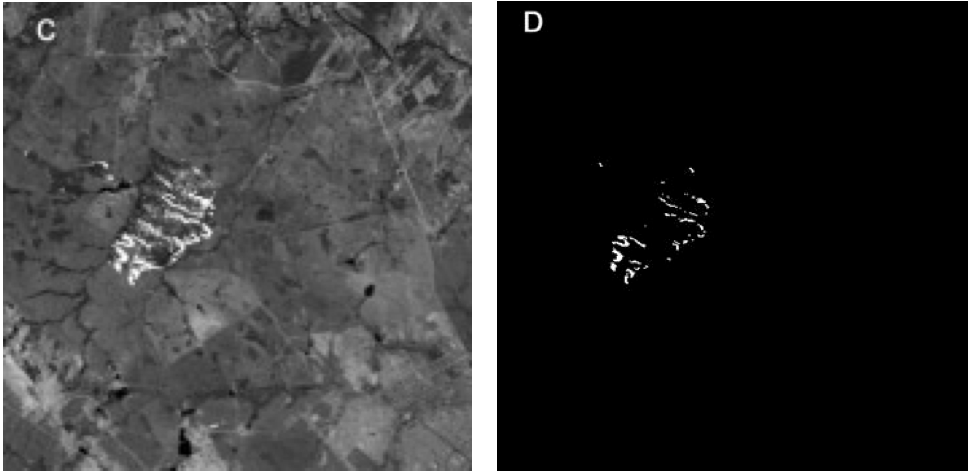
\includegraphics[width=3.5in]{eps/vodacek.png}\\
{\footnotesize Vodacek et al 2004}
\end{center}

We would like to use infrared imagery from aircraft to correct errors in the fire location.  Other
similar data is available from satellite imagery, but at much lower resolution.
%\end{figure}
\end{frame}

\begin{frame}
\frametitle{Testing the EnKF on a wildfire model}
A major component of the error in wildfire modeling is determining the 
\alert{position} of the fireline.  We want to test the behavior of the EnKF
under these conditions.\\
\vspace{.25in}
\hrule
\vspace{.25in}
Test procedure:
\begin{itemize}
\item Generate an ensemble by translating a single solution of the PDE model
randomly in space.
\item Use as data, a the temperature of a solution that is 
intentionally shifted away from the ensemble.
\end{itemize}
\end{frame}



\begin{frame}%
\frametitle{An example in 1D: filter degeneracy}%
\vspace{-.3in}
\begin{columns}%
\column[t]{.35\textwidth}%
\begin{center}Forecast ensemble\end{center}
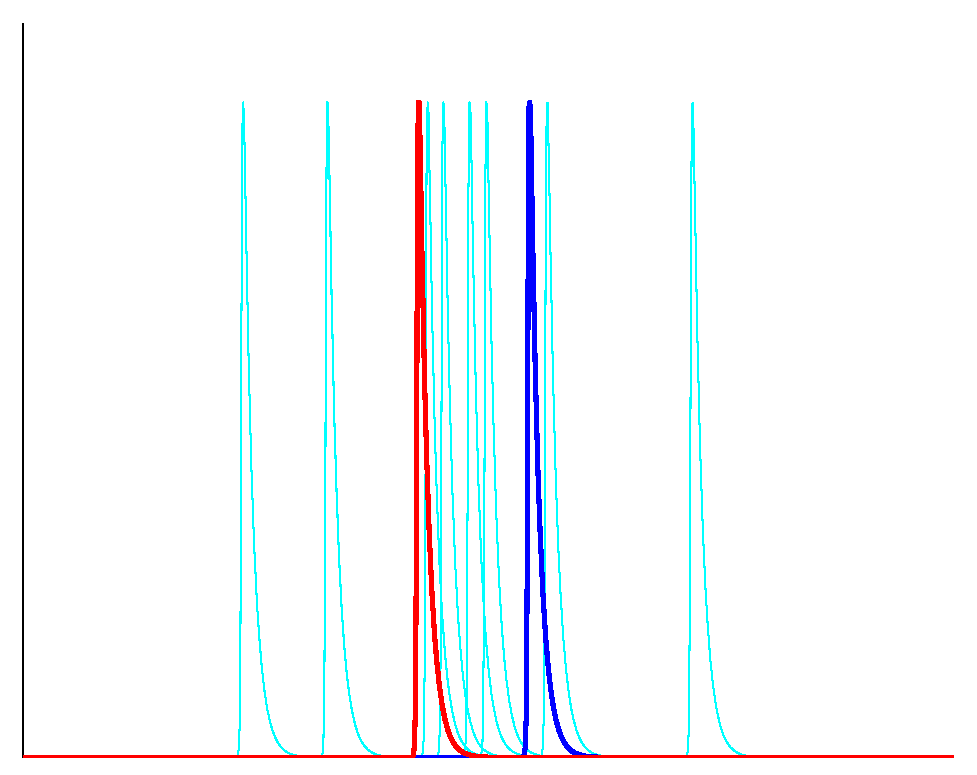
\includegraphics[height=.9in]{eps/tprior}
\begin{center}Analysis ensemble\end{center}
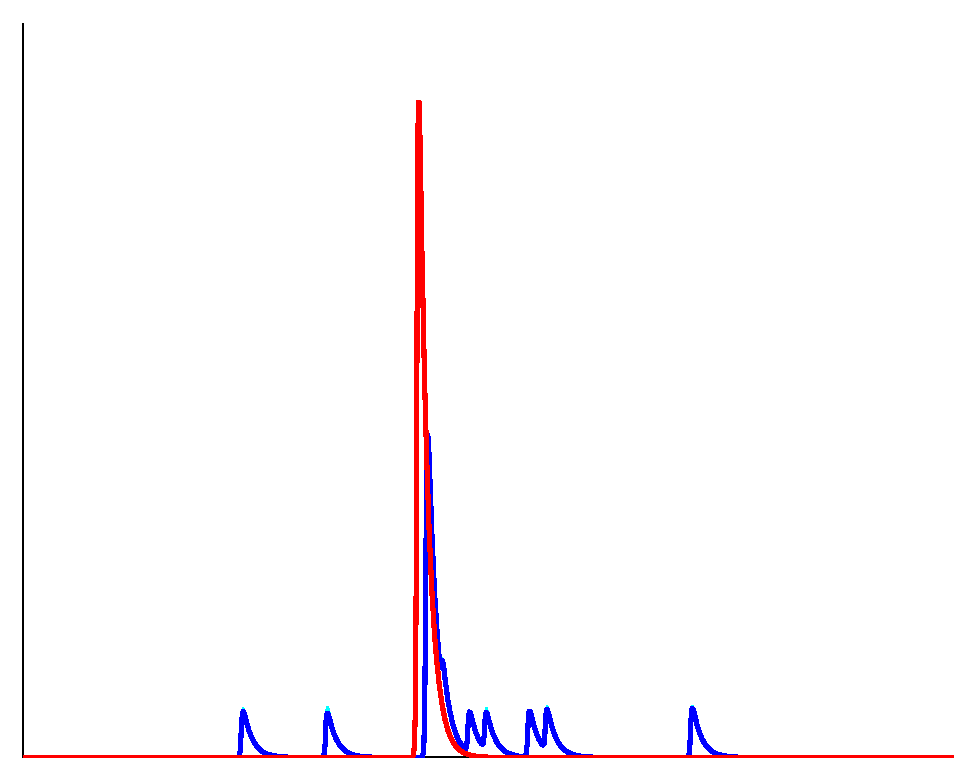
\includegraphics[height=.9in]{eps/tenkfeye}
\column[t]{.65\textwidth}
\vspace{.1in}
\begin{itemize}
\item
Ensemble size, $N=10$
\item
Forecast ensemble generated by translating by $N(0,\sigma^2)$, $\sigma^2=200$ $m^2$
\item
Identity observation function, $H=I$
\item
Data covariance, $R=10\mbox{tr}(P^f)I$
\end{itemize}
\vspace{.1in}
\begin{itemize}
\item
{\color{cyan}Cyan}: ensemble
\item
{\color{blue}Blue}: last ensemble member
\item
{\color{red}Red}: data
\end{itemize}
\vspace{.1in}
\begin{itemize}
\item
$\mbox{tr}(P^f)=4.7\times 10^6$
\item
$\mbox{tr}(P^a)=4.8\times 10^2$
\end{itemize}
\end{columns}
\end{frame}

\begin{frame}%
\frametitle{An example in 2D: non-physical results}%
\vspace{-.3in}
\begin{columns}%
\column[t]{.33\textwidth}%
\begin{center}Forecast ensemble\end{center}
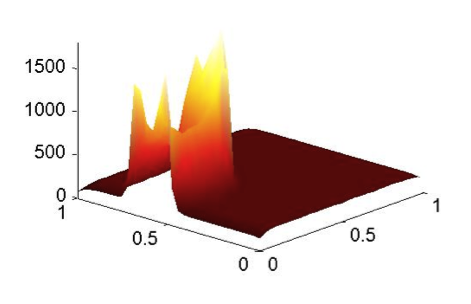
\includegraphics[height=1in]{eps/fire2d_prior}
\column[t]{.33\textwidth}%
\begin{center}Data\end{center}
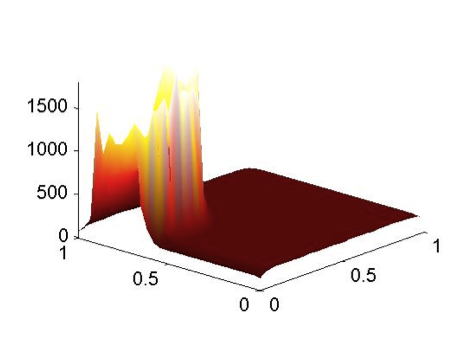
\includegraphics[height=1.1in]{eps/fire2d_data}
\column[t]{.33\textwidth}%
\begin{center}Analysis ensemble\end{center}
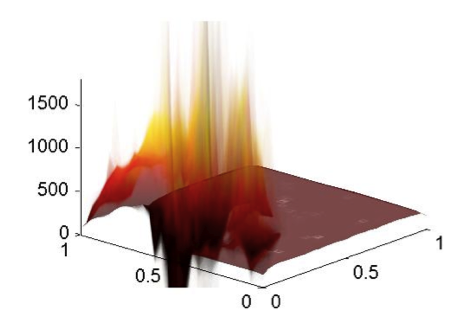
\includegraphics[height=1in]{eps/fire2d_post}
\end{columns}
\vspace{.1in}
\begin{itemize}
\item
Forecast ensemble generated by random spatial perturbations of the displayed image
\item
Analysis ensemble displayed as a superposition of semi-transparent images of each ensemble member
\item
Identity observation function, $H=I$
\item
Data variance, $100$ $K^2$
\end{itemize}
\end{frame}

%\section{Image registration}

%\subsection{Spatial errors}

\begin{frame}
\frametitle{What went wrong?}
\begin{columns}%
\column[t]{.6\textwidth}%
The Kalman update formula can be expressed as 
\[
X^a=A(X^f)^T,
\]
so $X^a_i\in\mbox{span}\{X^f\}$, where the analysis ensemble is made of \alert{linear combinations} of the forecast.
\vspace{.2in}
\column[t]{.4\textwidth}%
\begin{figure}[h]
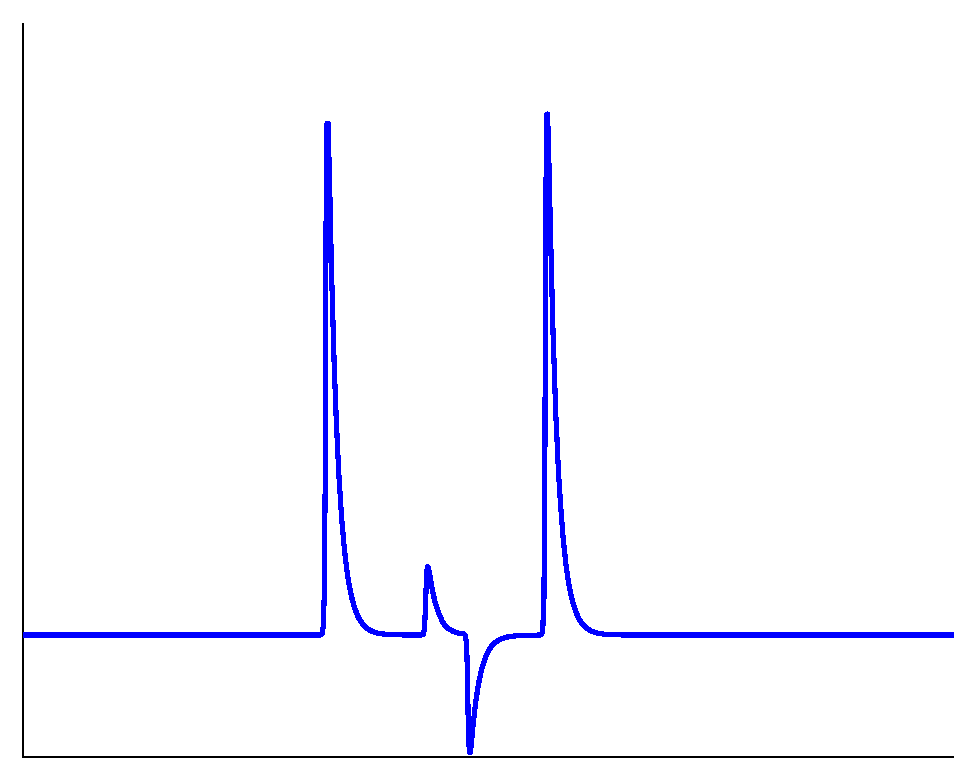
\includegraphics[height=1in]{eps/lincomb}
\end{figure}
\end{columns}
\hrule
\vspace{.2in}
Need to represent the \alert{position} of the fire as well as its \alert{shape}.
\end{frame}

\begin{frame}
\frametitle{Representing spatial error, in 1D}

\begin{columns}%
\column[t]{.35\textwidth}%
\vspace{-.5in}
%\begin{center}Forecast ensemble\end{center}
\begin{figure}[h]
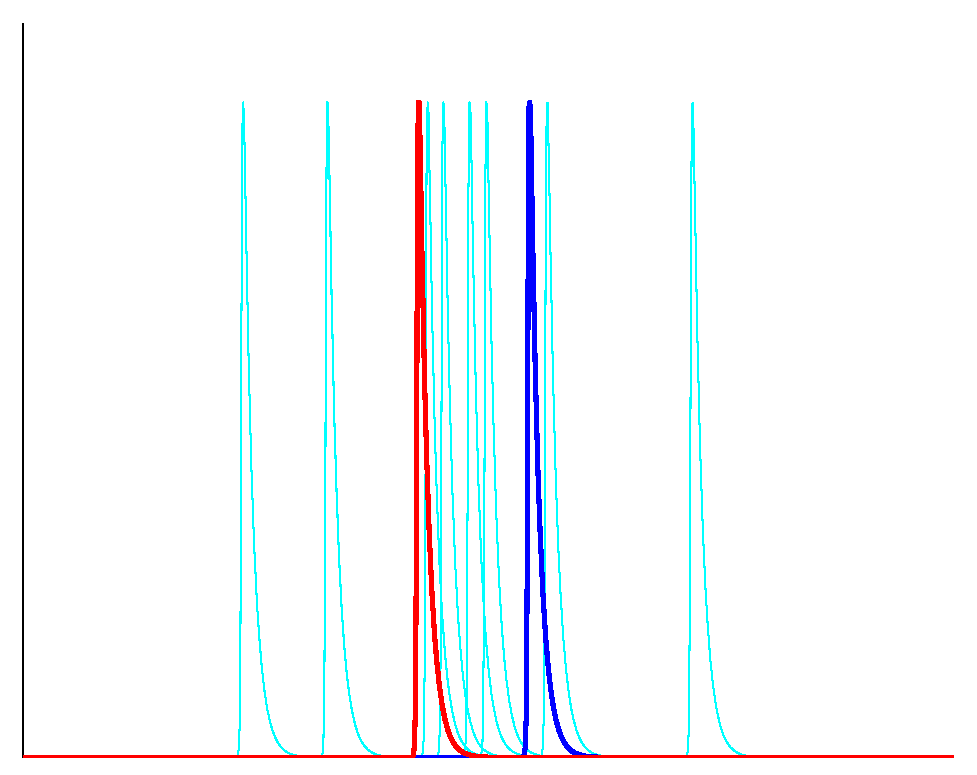
\includegraphics[height=1.25in]{eps/tprior}\\
\vspace{.05in}
%\begin{center}Analysis ensemble\end{center}
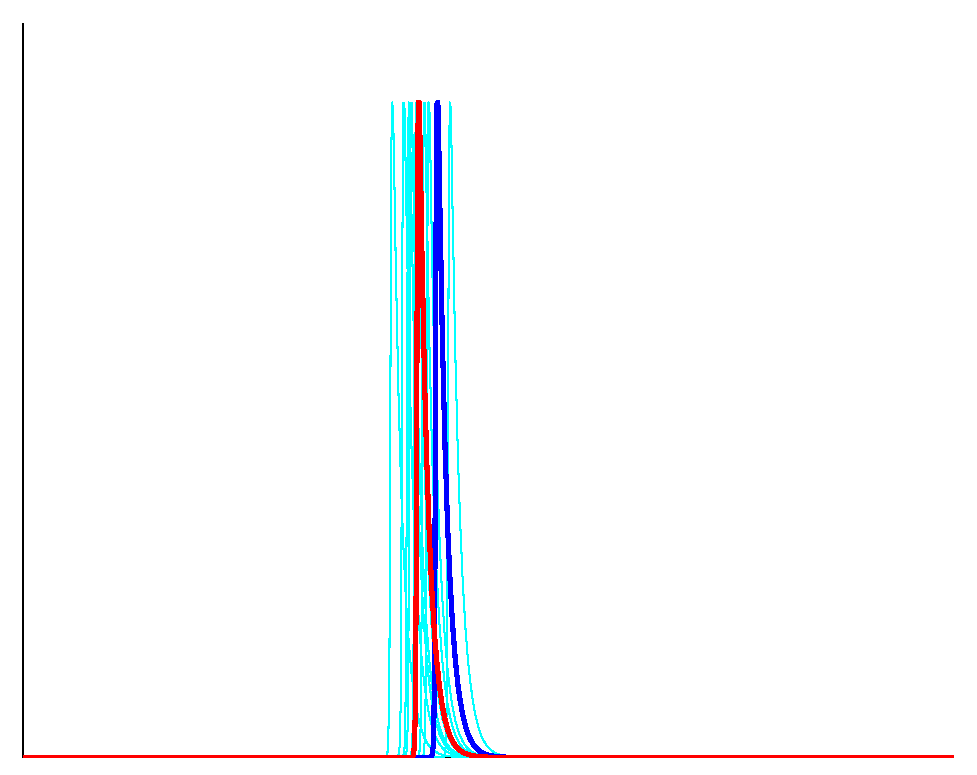
\includegraphics[height=1.25in]{eps/tenkfmorph}
\end{figure}
\column[t]{.65\textwidth}
\vspace{-.2in}
\begin{block}{Define a non-linear transformation}
$\mathcal{T}(u_i)=\mbox{argmax}\{u_0\}-\mbox{argmax}\{u_i\}=t_i$\\
$\mathcal{T}^{-1}(t_i)=u_0(x+t_i)=u_i$
\end{block}
\begin{itemize}
\item
$t_i$, translation of ensemble member $i$ from a ``reference'' state $u_0$
\item
run the EnKF with scalar ensemble $t_i$ and data $\mathcal{T}(Y)$
\item
recover analysis ensemble by applying the inverse transformation
\item
$t_i\sim \mathcal{N}(m,\sigma)$, by original construction of forecast ensemble
\end{itemize}
\end{columns}
\begin{center}But what about 2D?\end{center}
\end{frame}



\section{The morphing EnKF}

\begin{frame}
\frametitle{Overview of the morphing EnKF}
\begin{center}
\tikzstyle{decision} = [diamond, draw, fill=blue!20, 
    text width=4.5em, text badly centered, node distance=3cm, inner sep=0pt, scale=1]
\tikzstyle{block} = [rectangle, draw, fill=blue!20, 
    text width=8em, text centered, rounded corners, minimum height=4em, scale=1]
\tikzstyle{tblock} = [rectangle, draw, fill=yellow!20, 
    text width=8em, text centered, rounded corners, minimum height=4em, scale=1]
\tikzstyle{line} = [draw, -latex']
\tikzstyle{cloud} = [draw, ellipse,fill=red!20, node distance=3cm,
    minimum height=2em, text width=4.5em, text centered, scale=1]
\tikzstyle{refs} = [draw, ellipse,fill=green!20, node distance=3cm,
    minimum height=2em, text width=4.5em, text centered, scale=1]
\tikzstyle{inits} = [draw, ellipse,fill=green!20, node distance=3cm,
    minimum height=2em, text width=4.5em, text centered, scale=1]
{\tiny
\begin{tikzpicture}[node distance = 3cm, auto, scale=1]
\node [block] (model) {Model};
\node [tblock, right of=model] (ftrans) {Forward\\transformation};
\node [block, right of=ftrans] (enkf) {EnKF};
\node [tblock, above of=enkf, yshift=-1.5cm] (dtrans) {Data\\transformation};
\node [cloud, left of=dtrans, xshift=1cm] (data) {Data};
\node [refs, above of=ftrans] (ref) {Reference};
\node [tblock, above of=ref, yshift=-1.5cm] (itrans) {Inverse\\transformation};
\node [inits, above of=itrans, yshift=-1.75cm] (init) {Random Fields};
%\node [right of=ftrans] (rftrans) {};
\path [line] (model) -- (ftrans);
\path [line] (ftrans) -- (enkf);
\path [line] (enkf) -| ++(1.5cm,0cm) |- (itrans);
\path [line] (data) -- (dtrans);
\path [line] (itrans) -| ++(-4.5cm,-3cm) |- (model);
\path [line] (dtrans) -- (enkf);
\path [line] (ref) -- (ftrans);
\path [line] (ref) -| (dtrans);
\path [line] (model) |- (ref);
\path [line] (ref) -- (itrans);
\path [line] (init) -- (itrans);
\draw (model) ++(-1.5cm,2.75cm) node[anchor=west] {$\left[X^a\right]$};
\draw (model) ++(1.5cm,0cm) node[anchor=south] {$\left[X^f\right]$};
\draw (ftrans) ++(1.5cm,0cm) node[anchor=south] {$\left[T^f;R^f\right]$};
\draw (ref) ++(0cm,.75cm) node[anchor=west] {$u_0$};
\draw (dtrans) ++(0cm,.75cm) node[anchor=east] {$u_0$};
\draw (ftrans) ++(0cm,.75cm) node[anchor=east] {$u_0$};
\draw (enkf) ++(1.5cm,2.75cm) node[anchor=east] {$\left[T^a;R^a\right]$};
\draw (data) ++(.85cm,0cm) node[anchor=south] {$d$};
\draw (enkf) ++(0cm,.75cm) node[anchor=west] {$\left[T^d;r^d\right]$};
\draw (init) ++(0cm,-.6cm) node[anchor=west] {$\left[T^0;r^0\right]$};
\draw (ref) ++(-1.75cm,0cm) node[anchor=south] {Central solution};
\end{tikzpicture}}
\end{center}
\end{frame}

\begin{frame}
\frametitle{Morphing functions}
\begin{itemize}
\item
A \alert{morphing function}, $(I+T):\Omega\rightarrow\Omega$ defines a spatial perturbation of an image, $u$.  
\item
It is \alert{invertible} when $(I+T)^{-1}$ exists.
\item
An image $u$ ``morphed'' by $T$ is defined as $\tilde{u}(x)=u(x+Tx)=u\circ(I+T)(x)$.
\end{itemize}


\rule{\textwidth}{1pt}
\begin{table}[h]
\begin{tabular}{ccccc}
%\column{.25\textwidth}
$u$&$\circ$&$I+T$&$=$&$\tilde{u}$\\
%\begin{figure}[h]
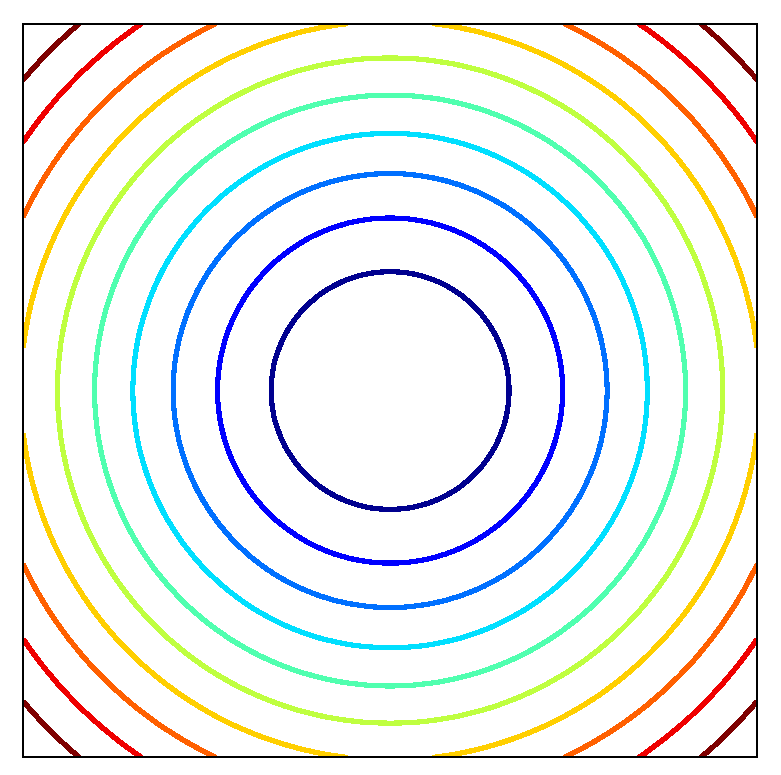
\includegraphics[height=1.in]{eps/morphorig}&&
%\end{figure}&skdf&
%\column{.125\textwidth}
%\column{.25\textwidth}
%\begin{figure}[h]
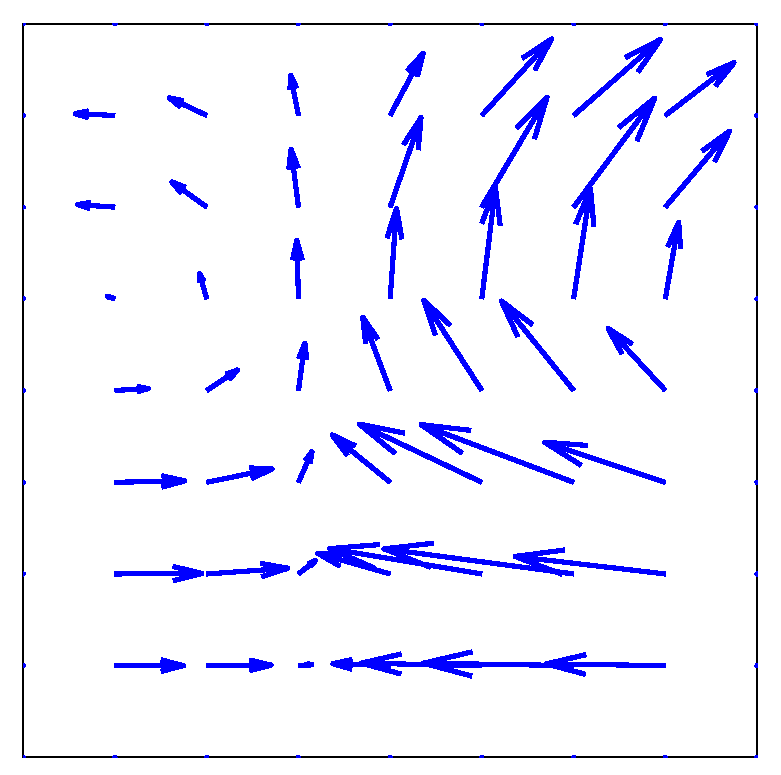
\includegraphics[height=1.in]{eps/morphfun}&&
%\end{figure}&sdfj&
%\column{.25\textwidth}
%\[\tilde{u}\]
%\begin{figure}[h]
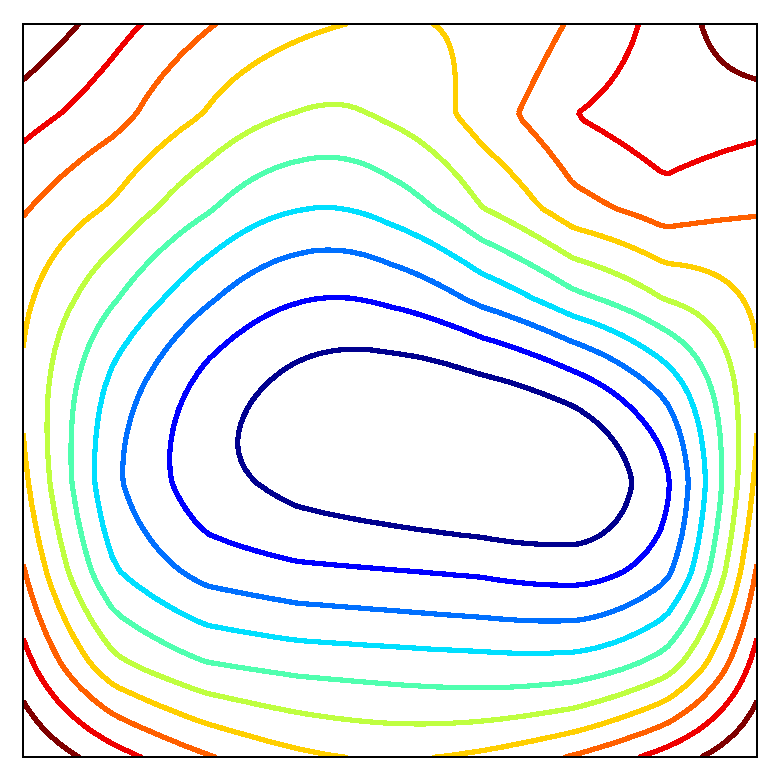
\includegraphics[height=1.in]{eps/morphtrans}
%\end{figure}

\end{tabular}
\end{table}
\end{frame}

%\subsection{Registration minimization}

\begin{frame}
\frametitle{Image registration}
Goal: Given two images $u$ and $v$, find an invertible morphing function, $T$, which makes $u\circ(I+T)\approx v$, while ensuring that $T$ is ``small'' as possible.
\begin{block}{Image registration problem}
\[
J_{u\rightarrow v}(T)=||u\circ(I+T)-v||_\mathcal{R}+||T||_\mathcal{T}\rightarrow\min_T
\]
\end{block}
\begin{itemize}
\item
$||r||_\mathcal{R}=c_\mathcal{R}||r||_2$
\item
$||T||_\mathcal{T}=c_\mathcal{T}||T||_2+c_\nabla||\nabla T||_2$
\item
$c_\mathcal{R}$, $c_\mathcal{T}$, and $c_\nabla$ are treated as optimization parameters
\end{itemize}
%\begin{block}{Morphing ensemble transformation}

%$\mathcal{T}(u_i)=\mbox{arg}\min_{T}\left\{ ||u_0\circ(I+T)^{-1}-u_i||_\mathcal{R}+||T||_\mathcal{M}\right\}$\\
%$\mathcal{T}^{-1}([T_i,r_i])=$
%\end{block}
\end{frame}

\begin{frame}
\frametitle{Minimizing the objective function}
\begin{columns}[t]
\column{.4\textwidth}
\vspace{-.3in}
\begin{figure}[h]
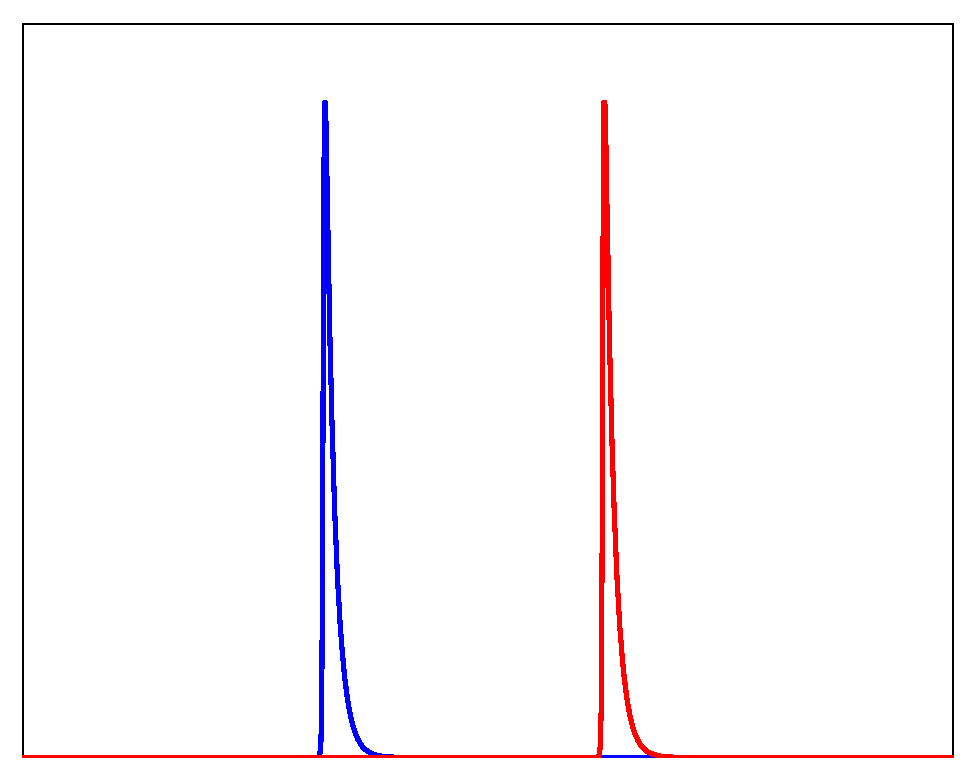
\includegraphics[height=1in]{eps/reggrad}
\end{figure}
\begin{center}$\nabla J_{u\rightarrow v}(0)=0$!!!\end{center}
\column{.6\textwidth}
Problems with minimization:
\begin{itemize}
\item{Highly nonlinear}
\item{Many local minima}
\item{Need an automated procedure}
\item{Needs to be done quickly}
\end{itemize}
\end{columns}
\vspace{.1in}
\rule{\textwidth}{1pt}
\vspace{.1in}
\begin{center}Steepest descent methods \alert{do not work} in general.\end{center}
\end{frame}

{\small
\begin{frame}
\frametitle{Summary of the algorithm}
Finding an acceptable solution requires a combination of standard techniques:
\begin{itemize}
\item \alert{Grid refinement}: Solve the problem only approximately at first, then refine
the solution on increasingly smaller sub-domains.
\item \alert{Sampling}:  Probe the feasibility region to escape local minima.
\item \alert{Image smoothing}: Smooth out sharp features of the images.
\item \alert{Levenberg-Marquardt}: Least-square descent method designed for nonlinear problems.
\end{itemize}
\end{frame}}

\begin{frame}
\begin{center}
\begin{columns}[c]
%\column{.25\textwidth}
\column{.3\textwidth}
\[u_0\]
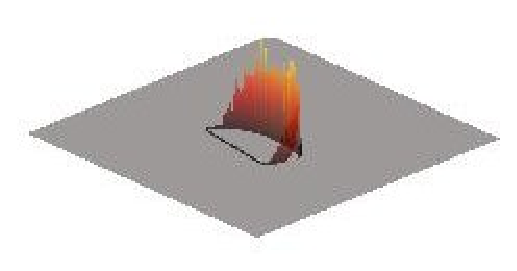
\includegraphics[width=1.25in]{eps/mtrans_u0}
\column{.7\textwidth}
\begin{block}{Morphing transformation}{\small
forward: $\mathcal{M}_{u_0}[u_i]=\left\{\begin{array}{l}
T_i,\quad\mbox{from registration}\\
r_i=u_i\circ(I+T_i)^{-1}-u_0
\end{array}\right.$\\
\vspace{.1in}
inverse: $\mathcal{M}_{u_0}^{-1}[T_i;r_i]=(u_0+r_i)\circ(I+T_i)$}
\end{block}
\end{columns}
\end{center}
\hspace{-.3in}\begin{tabular}{ccccccc}
&$[u_i]$&$\overset{u_0}{\longleftrightarrow}$&$[T_i$&;&$r_i]$&\\
\\
&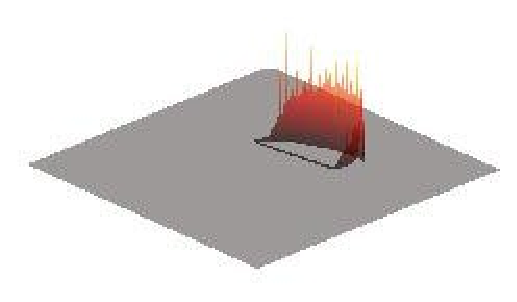
\includegraphics[width=1.25in]{eps/mtrans_u}&&
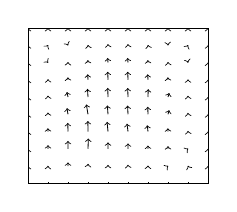
\begin{tikzpicture}[scale=.6]

\begin{axis}[%
name=main plot,%
axis on top,%
width=1.5in,%
scale only axis,%
xmin=0, xmax=2.514,%
ymin=0, ymax=2.514,%
ticks=none%
]
\addplot [->,color=black,solid,line width=0.5pt] coordinates{ (0,0) (0,0) };
\addplot [->,color=black,solid,line width=0.5pt] coordinates{ (0.279333,0) (0.279333,0) };
\addplot [->,color=black,solid,line width=0.5pt] coordinates{ (0.558667,0) (0.558667,0) };
\addplot [->,color=black,solid,line width=0.5pt] coordinates{ (0.838,0) (0.838,0) };
\addplot [->,color=black,solid,line width=0.5pt] coordinates{ (1.11733,0) (1.11733,0) };
\addplot [->,color=black,solid,line width=0.5pt] coordinates{ (1.39667,0) (1.39667,0) };
\addplot [->,color=black,solid,line width=0.5pt] coordinates{ (1.676,0) (1.676,0) };
\addplot [->,color=black,solid,line width=0.5pt] coordinates{ (1.95533,0) (1.95533,0) };
\addplot [->,color=black,solid,line width=0.5pt] coordinates{ (2.23467,0) (2.23467,0) };
\addplot [->,color=black,solid,line width=0.5pt] coordinates{ (2.514,0) (2.514,0) };
\addplot [->,color=black,solid,line width=0.5pt] coordinates{ (0,0.279333) (0,0.279333) };
\addplot [->,color=black,solid,line width=0.5pt] coordinates{ (0.279333,0.279333) (0.279411,0.281576) };
\addplot [->,color=black,solid,line width=0.5pt] coordinates{ (0.558667,0.279333) (0.558426,0.337635) };
\addplot [->,color=black,solid,line width=0.5pt] coordinates{ (0.838,0.279333) (0.840192,0.314578) };
\addplot [->,color=black,solid,line width=0.5pt] coordinates{ (1.11733,0.279333) (1.11738,0.296516) };
\addplot [->,color=black,solid,line width=0.5pt] coordinates{ (1.39667,0.279333) (1.39499,0.299243) };
\addplot [->,color=black,solid,line width=0.5pt] coordinates{ (1.676,0.279333) (1.67613,0.286073) };
\addplot [->,color=black,solid,line width=0.5pt] coordinates{ (1.95533,0.279333) (1.95697,0.280668) };
\addplot [->,color=black,solid,line width=0.5pt] coordinates{ (2.23467,0.279333) (2.23443,0.279966) };
\addplot [->,color=black,solid,line width=0.5pt] coordinates{ (2.514,0.279333) (2.514,0.279333) };
\addplot [->,color=black,solid,line width=0.5pt] coordinates{ (0,0.558667) (0,0.558667) };
\addplot [->,color=black,solid,line width=0.5pt] coordinates{ (0.279333,0.558667) (0.279096,0.617009) };
\addplot [->,color=black,solid,line width=0.5pt] coordinates{ (0.558667,0.558667) (0.558261,0.68472) };
\addplot [->,color=black,solid,line width=0.5pt] coordinates{ (0.838,0.558667) (0.842765,0.724556) };
\addplot [->,color=black,solid,line width=0.5pt] coordinates{ (1.11733,0.558667) (1.11741,0.662113) };
\addplot [->,color=black,solid,line width=0.5pt] coordinates{ (1.39667,0.558667) (1.39746,0.645082) };
\addplot [->,color=black,solid,line width=0.5pt] coordinates{ (1.676,0.558667) (1.67414,0.610122) };
\addplot [->,color=black,solid,line width=0.5pt] coordinates{ (1.95533,0.558667) (1.95408,0.600585) };
\addplot [->,color=black,solid,line width=0.5pt] coordinates{ (2.23467,0.558667) (2.23606,0.559774) };
\addplot [->,color=black,solid,line width=0.5pt] coordinates{ (2.514,0.558667) (2.514,0.558667) };
\addplot [->,color=black,solid,line width=0.5pt] coordinates{ (0,0.838) (0,0.838) };
\addplot [->,color=black,solid,line width=0.5pt] coordinates{ (0.279333,0.838) (0.278224,0.890743) };
\addplot [->,color=black,solid,line width=0.5pt] coordinates{ (0.558667,0.838) (0.55513,0.976672) };
\addplot [->,color=black,solid,line width=0.5pt] coordinates{ (0.838,0.838) (0.835746,1.0077) };
\addplot [->,color=black,solid,line width=0.5pt] coordinates{ (1.11733,0.838) (1.10431,0.993482) };
\addplot [->,color=black,solid,line width=0.5pt] coordinates{ (1.39667,0.838) (1.38263,0.96421) };
\addplot [->,color=black,solid,line width=0.5pt] coordinates{ (1.676,0.838) (1.66538,0.938617) };
\addplot [->,color=black,solid,line width=0.5pt] coordinates{ (1.95533,0.838) (1.95321,0.890148) };
\addplot [->,color=black,solid,line width=0.5pt] coordinates{ (2.23467,0.838) (2.23374,0.848051) };
\addplot [->,color=black,solid,line width=0.5pt] coordinates{ (2.514,0.838) (2.514,0.838) };
\addplot [->,color=black,solid,line width=0.5pt] coordinates{ (0,1.11733) (0,1.11733) };
\addplot [->,color=black,solid,line width=0.5pt] coordinates{ (0.279333,1.11733) (0.277552,1.14545) };
\addplot [->,color=black,solid,line width=0.5pt] coordinates{ (0.558667,1.11733) (0.54399,1.21598) };
\addplot [->,color=black,solid,line width=0.5pt] coordinates{ (0.838,1.11733) (0.814536,1.27541) };
\addplot [->,color=black,solid,line width=0.5pt] coordinates{ (1.11733,1.11733) (1.10812,1.25959) };
\addplot [->,color=black,solid,line width=0.5pt] coordinates{ (1.39667,1.11733) (1.3904,1.25713) };
\addplot [->,color=black,solid,line width=0.5pt] coordinates{ (1.676,1.11733) (1.67218,1.238) };
\addplot [->,color=black,solid,line width=0.5pt] coordinates{ (1.95533,1.11733) (1.97148,1.18296) };
\addplot [->,color=black,solid,line width=0.5pt] coordinates{ (2.23467,1.11733) (2.23231,1.1388) };
\addplot [->,color=black,solid,line width=0.5pt] coordinates{ (2.514,1.11733) (2.514,1.11733) };
\addplot [->,color=black,solid,line width=0.5pt] coordinates{ (0,1.39667) (0,1.39667) };
\addplot [->,color=black,solid,line width=0.5pt] coordinates{ (0.279333,1.39667) (0.277781,1.41807) };
\addplot [->,color=black,solid,line width=0.5pt] coordinates{ (0.558667,1.39667) (0.543756,1.47643) };
\addplot [->,color=black,solid,line width=0.5pt] coordinates{ (0.838,1.39667) (0.830724,1.52827) };
\addplot [->,color=black,solid,line width=0.5pt] coordinates{ (1.11733,1.39667) (1.11347,1.54322) };
\addplot [->,color=black,solid,line width=0.5pt] coordinates{ (1.39667,1.39667) (1.39235,1.5423) };
\addplot [->,color=black,solid,line width=0.5pt] coordinates{ (1.676,1.39667) (1.67855,1.52349) };
\addplot [->,color=black,solid,line width=0.5pt] coordinates{ (1.95533,1.39667) (1.97219,1.46123) };
\addplot [->,color=black,solid,line width=0.5pt] coordinates{ (2.23467,1.39667) (2.23324,1.41671) };
\addplot [->,color=black,solid,line width=0.5pt] coordinates{ (2.514,1.39667) (2.514,1.39667) };
\addplot [->,color=black,solid,line width=0.5pt] coordinates{ (0,1.676) (0,1.676) };
\addplot [->,color=black,solid,line width=0.5pt] coordinates{ (0.279333,1.676) (0.279002,1.68477) };
\addplot [->,color=black,solid,line width=0.5pt] coordinates{ (0.558667,1.676) (0.556058,1.71489) };
\addplot [->,color=black,solid,line width=0.5pt] coordinates{ (0.838,1.676) (0.833382,1.7641) };
\addplot [->,color=black,solid,line width=0.5pt] coordinates{ (1.11733,1.676) (1.11326,1.80515) };
\addplot [->,color=black,solid,line width=0.5pt] coordinates{ (1.39667,1.676) (1.39258,1.80535) };
\addplot [->,color=black,solid,line width=0.5pt] coordinates{ (1.676,1.676) (1.67094,1.76413) };
\addplot [->,color=black,solid,line width=0.5pt] coordinates{ (1.95533,1.676) (1.95229,1.71457) };
\addplot [->,color=black,solid,line width=0.5pt] coordinates{ (2.23467,1.676) (2.23458,1.68199) };
\addplot [->,color=black,solid,line width=0.5pt] coordinates{ (2.514,1.676) (2.514,1.676) };
\addplot [->,color=black,solid,line width=0.5pt] coordinates{ (0,1.95533) (0,1.95533) };
\addplot [->,color=black,solid,line width=0.5pt] coordinates{ (0.279333,1.95533) (0.27993,1.95455) };
\addplot [->,color=black,solid,line width=0.5pt] coordinates{ (0.558667,1.95533) (0.558763,1.96232) };
\addplot [->,color=black,solid,line width=0.5pt] coordinates{ (0.838,1.95533) (0.835408,1.99323) };
\addplot [->,color=black,solid,line width=0.5pt] coordinates{ (1.11733,1.95533) (1.11165,2.02835) };
\addplot [->,color=black,solid,line width=0.5pt] coordinates{ (1.39667,1.95533) (1.39096,2.0287) };
\addplot [->,color=black,solid,line width=0.5pt] coordinates{ (1.676,1.95533) (1.67283,1.99342) };
\addplot [->,color=black,solid,line width=0.5pt] coordinates{ (1.95533,1.95533) (1.95485,1.96231) };
\addplot [->,color=black,solid,line width=0.5pt] coordinates{ (2.23467,1.95533) (2.23488,1.95435) };
\addplot [->,color=black,solid,line width=0.5pt] coordinates{ (2.514,1.95533) (2.514,1.95533) };
\addplot [->,color=black,solid,line width=0.5pt] coordinates{ (0,2.23467) (0,2.23467) };
\addplot [->,color=black,solid,line width=0.5pt] coordinates{ (0.279333,2.23467) (0.279645,2.23522) };
\addplot [->,color=black,solid,line width=0.5pt] coordinates{ (0.558667,2.23467) (0.559081,2.2337) };
\addplot [->,color=black,solid,line width=0.5pt] coordinates{ (0.838,2.23467) (0.837657,2.23735) };
\addplot [->,color=black,solid,line width=0.5pt] coordinates{ (1.11733,2.23467) (1.11588,2.2527) };
\addplot [->,color=black,solid,line width=0.5pt] coordinates{ (1.39667,2.23467) (1.39522,2.25303) };
\addplot [->,color=black,solid,line width=0.5pt] coordinates{ (1.676,2.23467) (1.67553,2.23723) };
\addplot [->,color=black,solid,line width=0.5pt] coordinates{ (1.95533,2.23467) (1.95543,2.23358) };
\addplot [->,color=black,solid,line width=0.5pt] coordinates{ (2.23467,2.23467) (2.23495,2.23525) };
\addplot [->,color=black,solid,line width=0.5pt] coordinates{ (2.514,2.23467) (2.514,2.23467) };
\addplot [->,color=black,solid,line width=0.5pt] coordinates{ (0,2.514) (0,2.514) };
\addplot [->,color=black,solid,line width=0.5pt] coordinates{ (0.279333,2.514) (0.279333,2.514) };
\addplot [->,color=black,solid,line width=0.5pt] coordinates{ (0.558667,2.514) (0.558667,2.514) };
\addplot [->,color=black,solid,line width=0.5pt] coordinates{ (0.838,2.514) (0.838,2.514) };
\addplot [->,color=black,solid,line width=0.5pt] coordinates{ (1.11733,2.514) (1.11733,2.514) };
\addplot [->,color=black,solid,line width=0.5pt] coordinates{ (1.39667,2.514) (1.39667,2.514) };
\addplot [->,color=black,solid,line width=0.5pt] coordinates{ (1.676,2.514) (1.676,2.514) };
\addplot [->,color=black,solid,line width=0.5pt] coordinates{ (1.95533,2.514) (1.95533,2.514) };
\addplot [->,color=black,solid,line width=0.5pt] coordinates{ (2.23467,2.514) (2.23467,2.514) };
\addplot [->,color=black,solid,line width=0.5pt] coordinates{ (2.514,2.514) (2.514,2.514) };
\end{axis}

\end{tikzpicture}
&&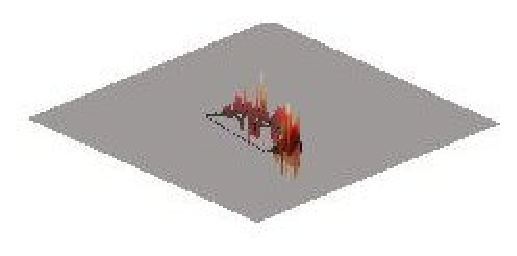
\includegraphics[width=1.25in]{eps/mtrans_r}&
\end{tabular}
\end{frame}

\begin{frame}
%\frametitle{The morphing transformation}
%\vspace{-.1in}
Linear combinations of transformed states consist of a single fire moving in space.
\begin{figure}[h]
\begin{tabular}{c|ccc|c}
$u_0$&\multicolumn{3}{c|}{Intermediate states $\mathcal{M}_{u_0}^{-1}
[\lambda T_i,\lambda r_i]$}&$u_i$ \\
\fbox{\includegraphics[height=.55in]{eps/lc_5}}&
\fbox{\includegraphics[height=.55in]{eps/lc_good_4}}&
\fbox{\includegraphics[height=.55in]{eps/lc_good_3}}&
\fbox{\includegraphics[height=.55in]{eps/lc_good_2}}&
\fbox{\includegraphics[height=.55in]{eps/lc_1}} \\
$\lambda=0$&$1/4$&$1/2$&$3/4$&$1$ 
\end{tabular}
\end{figure}
\end{frame}

\begin{frame}[fragile]
%\frametitle{An aside}
\vspace{-.1in}
Why use $r=u\circ(I+T)^{-1}-u_0$ instead of $\tilde{r}=u-u_0\circ(I+T)$?\\
\vspace{-.1in}
\begin{columns}[c]
\column{.2\textwidth}
%\vspace{1in}
\begin{align*}
T(x)&=1\\
{\color{blue}u(x)}&=\varphi(x)\\
{\color{red}u_0(x)}&=2\varphi(x+1)
\end{align*}
\column{.4\textwidth}
{\scriptsize
\begin{align*}
\tilde{u}_\lambda(x) &= \varphi(x+\lambda)+
\underbrace{\lambda\varphi(x+1)}_{\mbox{``residual''}}
\end{align*}
\begin{center}
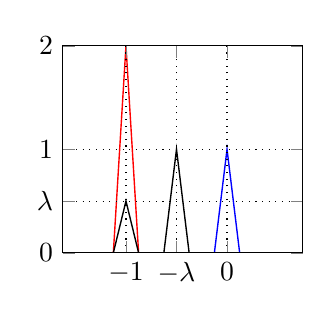
\begin{tikzpicture}

\pgfplotsset{every axis grid/.style={style=dotted}}


\begin{axis}[%
name=main plot,%
axis on top,%
width=1.2in,%
scale only axis,%
xtick={6,10,14},%
xticklabels={$-1$,$-\lambda$,$0$},%
ytick={0,0.5,1,2},%
yticklabels={$0$,$\lambda$,$1$,$2$},%
xmajorgrids,ymajorgrids,enlargelimits=false]%

\addplot [%
color=red,%
solid,%
line width=0.5pt%
] coordinates{
 (5,0) (6,2) (7,0)
};

\addplot [%
color=blue,%
solid,%
line width=0.5pt%
] coordinates{
 (13,0) (14,1) (15,0)
};

\addplot [%
color=black,%
solid,%
line width=0.5pt%
] coordinates{
(1,0) (5,0) (6,0.5) (7,0) (9,0) (10,1) (11,0) (20,0)
};

\end{axis}

\end{tikzpicture}

\end{center}}
\column{.4\textwidth}
%\begin{center}
%\vspace{-.2in}
%\begin{flushright}
{\scriptsize
\begin{align*}
u_\lambda(x)&= \varphi(x+\lambda)
+\underbrace{\lambda\varphi(x+\lambda)}_{\mbox{``residual''}}
\end{align*}
\begin{center}
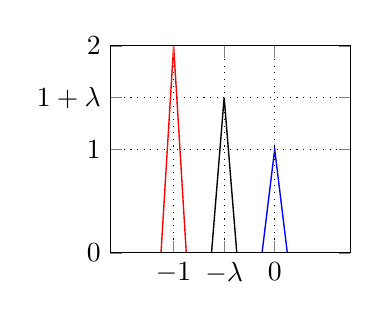
\begin{tikzpicture}

\pgfplotsset{every axis grid/.style={style=dotted}}


\begin{axis}[%
name=main plot,%
axis on top,%
width=1.2in,%
scale only axis,%
xtick={6,10,14},%
xticklabels={$-1$,$-\lambda$,$0$},%
ytick={0,1,1.5,2},%
yticklabels={$0$,$1$,$1+\lambda$,$2$},%
xmajorgrids,ymajorgrids,enlargelimits=false]%

\addplot [%
color=red,%
solid,%
line width=0.5pt%
] coordinates{
 (5,0) (6,2) (7,0)
};

\addplot [%
color=blue,%
solid,%
line width=0.5pt%
] coordinates{
 (13,0) (14,1) (15,0)
};

\addplot [%
color=black,%
solid,%
line width=0.5pt%
] coordinates{
(1,0) (9,0) (10,1.5) (11,0) (20,0)
};

\end{axis}

\end{tikzpicture}

\end{center}}
%\end{flushright}
%\end{center}
\end{columns}
\vspace{.2in}
\begin{center}
$\tilde{u}_\lambda$: the residual component remains \alert{fixed} in space.  \\
$u_\lambda$: the residual component \alert{moves} with the image.
\end{center}
\end{frame}

\begin{frame}
\[\tilde{\mathcal{M}}_{u_0}^{-1}[\lambda T,\lambda \tilde{r}]=u_0\circ(I+\lambda T)+
\overbrace{\lambda (u-u_0\circ(I+T))}^{\mbox{``residual''}}
\]
\vspace{-.5in}
\begin{figure}[h]
\begin{tabular}{c|ccc|c}
$\lambda=0$&$1/4$&$1/2$&$3/4$&$1$ \\
\includegraphics[height=.6in]{eps/lc_5}&
\includegraphics[height=.6in]{eps/lc_bad_4}&
\includegraphics[height=.6in]{eps/lc_bad_3}&
\includegraphics[height=.6in]{eps/lc_bad_2}&
\includegraphics[height=.6in]{eps/lc_1}\\
\includegraphics[height=.6in]{eps/lc_5}
&\includegraphics[height=.6in]{eps/lc_good_4}&
\includegraphics[height=.6in]{eps/lc_good_3}&
\includegraphics[height=.6in]{eps/lc_good_2}&
\includegraphics[height=.6in]{eps/lc_1}
\end{tabular}
\end{figure}
\[\mathcal{M}_{u_0}^{-1}[\lambda T,\lambda r]=
u_0\circ (I+\lambda T)+\underbrace{\lambda (u\circ (I+ T)^{-1}-u_0)\circ (I+\lambda T)}
_{\mbox{``residual''}}\]
\end{frame}

\begin{frame}
\begin{columns}[t]
\column{.4\textwidth}
\vspace{-.4in}
\[
\left[
\begin{array}{c}
u_1\\
u_2\\
\vdots\\
u_n
\end{array}
\right]\leftrightarrow
\left[
\begin{array}{c}
T\\
r_1\\
r_2\\
\vdots\\ 
r_n
\end{array}
\right]=\left[\begin{array}{c}T\\R\end{array}\right]
\]
\column{.6\textwidth}
For multi-variable states, register only one variable and use the registered morphing function to create a residual for each variable.
\end{columns}
\vspace{.2in}
\rule{\textwidth}{1pt}
\vspace{.2in}
\begin{columns}[t]
\column{.65\textwidth}
For $3D$ variables apply morphing function to each horizontal plane:  $u_i(:,:,k)$.
\column{.35\textwidth}
\vspace{-.5in}
\begin{figure}[h]
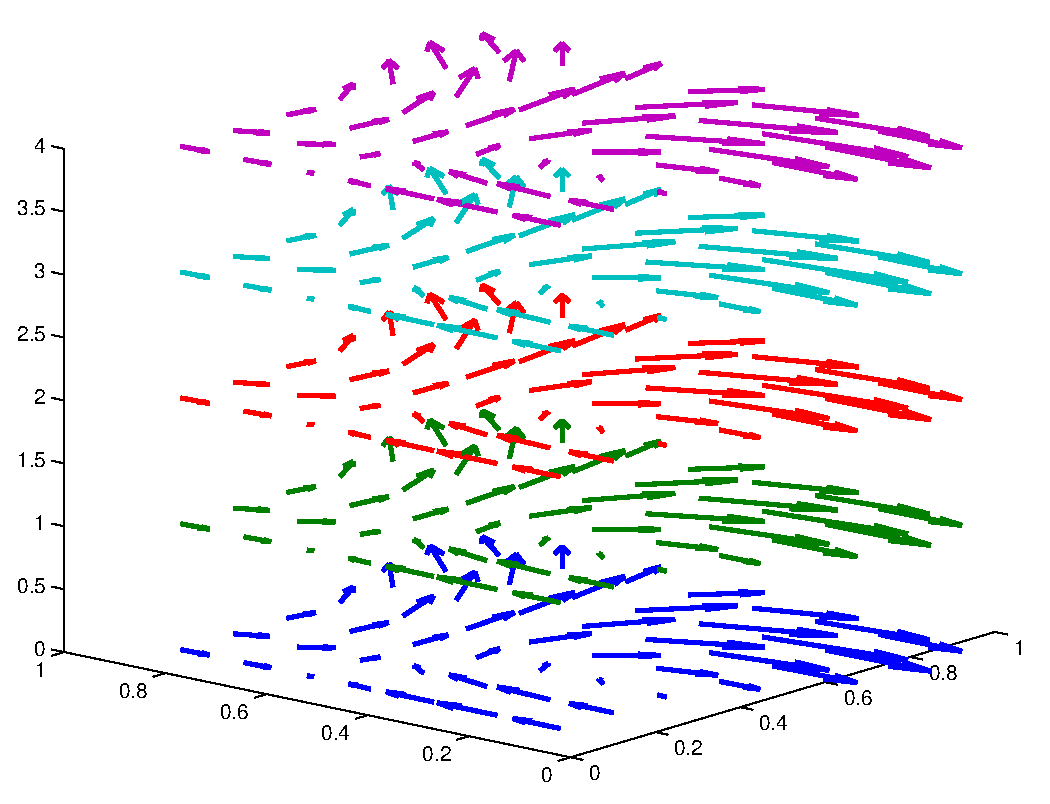
\includegraphics[height=1in]{eps/morph3d}
\end{figure}
\end{columns}
\end{frame}

\begin{frame}
\frametitle{Data transformation}
%\begin{columns}[c]
%\column{.5\textwidth}
\begin{tabular}{l|c|c|}
&Original&Transformed\\
Data&
$d$&$\left[T_d;r_d\right]$\\
&&\\
Observation function&
$h:
\left[
\begin{array}{c}
u_1\\
\vdots\\
u_n
\end{array}
\right]\mapsto \left[u_1\right]$&$\tilde{h}:
\left[
\begin{array}{c}
T\\
r_1\\
\vdots\\
r_n
\end{array}
\right]\mapsto \left[\begin{array}{c}T\\r_1\end{array}\right]$
\end{tabular}
\vspace{.1in}
\begin{itemize}
\item Data undergoes the same transformation, but only contains the registration variable.
\item Observation function is modified to act on the morphed ensemble states.
\item Can be extended to more general observations, but limited to ``image-like'' data that is a point wise function of the model variables.
\end{itemize}
%\end{columns}
\end{frame}

\begin{frame}
\frametitle{Initial ensemble}
\begin{columns}[c]
\column{.8\textwidth}
\begin{block}{Random Fields}
{\footnotesize
\[s_{j}\propto\mathcal{R}\mathrm{e}\left\{
\sum_{k=0}^{n-1}(c_{k}+id_{k})\left(\frac{k}{h}\right)^{-1-\alpha}
e^{2\pi i kj/n} \right\}\]
\[c_k,d_k\sim \mathcal{N}(0,1), \mbox{independent}\]}\end{block}
\begin{enumerate}
\item Choose a reference solution, $u_0$.
\item Generate random morphing function, $T$, out of random fields.
\item Generate random residuals, $R$, out of random fields for each variable.
\item $X^0_i\leftarrow \mathcal{M}^{-1}_{u_0}([T,R])$
\end{enumerate}
\column{.2\textwidth}
\begin{tabular}{c}
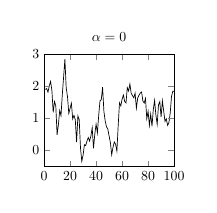
\begin{tikzpicture}[scale=.5]

% defining custom colors
\definecolor{mycolor1}{rgb}{0,0.5,0}
\definecolor{mycolor2}{rgb}{0,0.75,0.75}

\begin{axis}[%
name=main plot,%
axis on top,%
width=1.3in,%
scale only axis,%
title={$\alpha=0$},%
xmin=0, xmax=100,%
ymin=-0.5, ymax=3%
]
\addplot [%
color=black,%
solid,%
line width=0.5pt%
] coordinates{
 (1,1.90984) (2,1.93149) (3,1.82) (4,2.01912) (5,2.1557) (6,1.87108) (7,1.19167) (8,1.52743) (9,1.39428) (10,0.49032) (11,0.803212) (12,1.24708) (13,1.09064) (14,1.73826) (15,2.28701) (16,2.84891) (17,1.96058) (18,1.68214) (19,1.15765) (20,1.314) (21,1.4779) (22,0.985111) (23,1.09636) (24,0.961923) (25,0.258952) (26,1.0798) (27,0.966575) (28,0.0803523) (29,-0.335926) (30,-0.143213) (31,0.179485) (32,0.15306) (33,0.300251) (34,0.404592) (35,0.292909) (36,0.453005) (37,0.708517) (38,0.0680895) (39,0.510886) (40,0.822266) (41,0.548815) (42,1.09415) (43,1.55141) (44,1.59047) (45,1.97743) (46,1.22152) (47,0.925987) (48,0.736929) (49,0.673296) (50,0.455371) (51,0.247133) (52,-0.134345) (53,0.100075) (54,0.266151) (55,0.193883) (56,-0.0194579) (57,0.780512) (58,1.48556) (59,1.39295) (60,1.60174) (61,1.73049) (62,1.53012) (63,1.48631) (64,1.96299) (65,1.85749) (66,2.0754) (67,1.78265) (68,1.71334) (69,1.64471) (70,1.78636) (71,1.32276) (72,1.63914) (73,1.72561) (74,1.79309) (75,1.8283) (76,1.54254) (77,1.48138) (78,1.62363) (79,0.990405) (80,1.22209) (81,0.783005) (82,1.13488) (83,0.75532) (84,1.278) (85,1.56645) (86,1.10291) (87,0.817316) (88,1.42362) (89,1.52321) (90,1.04799) (91,1.55267) (92,1.22733) (93,0.908916) (94,0.986195) (95,0.784564) (96,0.869779) (97,1.16112) (98,1.68372) (99,1.85036) (100,1.84831)
};

\end{axis}

\end{tikzpicture}
\\
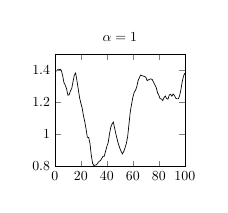
\begin{tikzpicture}[scale=.5]

% defining custom colors
\definecolor{mycolor1}{rgb}{0,0.5,0}
\definecolor{mycolor2}{rgb}{0,0.75,0.75}

\begin{axis}[%
name=main plot,%
axis on top,%
width=1.3in,%
scale only axis,%
title={$\alpha=1$},%
xmin=0, xmax=100,%
ymin=0.8, ymax=1.5%
]
\addplot [%
color=black,%
solid,%
line width=0.5pt%
] coordinates{
 (1,1.39564) (2,1.40349) (3,1.40447) (4,1.40789) (5,1.39976) (6,1.3675) (7,1.32351) (8,1.30785) (9,1.28571) (10,1.2451) (11,1.24745) (12,1.27145) (13,1.28793) (14,1.33108) (15,1.36997) (16,1.38347) (17,1.33482) (18,1.28354) (19,1.23045) (20,1.19611) (21,1.16565) (22,1.11705) (23,1.08041) (24,1.03472) (25,0.982214) (26,0.981452) (27,0.945084) (28,0.871921) (29,0.820809) (30,0.805831) (31,0.809208) (32,0.810379) (33,0.821301) (34,0.831834) (35,0.83672) (36,0.849572) (37,0.864069) (38,0.864273) (39,0.894683) (40,0.924726) (41,0.948749) (42,1.00078) (43,1.04504) (44,1.06614) (45,1.07745) (46,1.03888) (47,1.00165) (48,0.967231) (49,0.937585) (50,0.913842) (51,0.894181) (52,0.879041) (53,0.893874) (54,0.917538) (55,0.944726) (56,0.986581) (57,1.06398) (58,1.14118) (59,1.18808) (60,1.23166) (61,1.26268) (62,1.27528) (63,1.29675) (64,1.33503) (65,1.35543) (66,1.37103) (67,1.36714) (68,1.3645) (69,1.36274) (70,1.35629) (71,1.3361) (72,1.34134) (73,1.34522) (74,1.34699) (75,1.34191) (76,1.32472) (77,1.30868) (78,1.29253) (79,1.25961) (80,1.24459) (81,1.22271) (82,1.22207) (83,1.21244) (84,1.23057) (85,1.24034) (86,1.2239) (87,1.22022) (88,1.24617) (89,1.25126) (90,1.23905) (91,1.25289) (92,1.24311) (93,1.22624) (94,1.22236) (95,1.2224) (96,1.24324) (97,1.28146) (98,1.33092) (99,1.36519) (100,1.38302)
};

\end{axis}

\end{tikzpicture}
\\
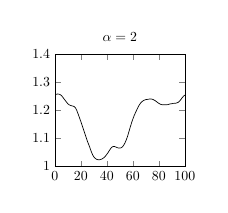
\begin{tikzpicture}[scale=.5]

% defining custom colors
\definecolor{mycolor1}{rgb}{0,0.5,0}
\definecolor{mycolor2}{rgb}{0,0.75,0.75}

\begin{axis}[%
name=main plot,%
axis on top,%
width=1.3in,%
scale only axis,%
title={$\alpha=2$},%
xmin=0, xmax=100,%
ymin=1, ymax=1.4%
]
\addplot [%
color=black,%
solid,%
line width=0.5pt%
] coordinates{
 (1,1.25737) (2,1.25851) (3,1.25826) (4,1.25674) (5,1.25341) (6,1.24799) (7,1.2415) (8,1.23557) (9,1.22967) (10,1.22377) (11,1.22005) (12,1.2181) (13,1.21656) (14,1.21563) (15,1.21349) (16,1.20816) (17,1.1984) (18,1.18634) (19,1.17323) (20,1.16008) (21,1.14672) (22,1.13258) (23,1.11856) (24,1.10439) (25,1.09067) (26,1.07905) (27,1.06662) (28,1.05339) (29,1.0422) (30,1.03431) (31,1.02919) (32,1.0259) (33,1.0244) (34,1.0241) (35,1.02467) (36,1.02642) (37,1.02909) (38,1.03246) (39,1.0376) (40,1.04359) (41,1.05014) (42,1.05771) (43,1.0645) (44,1.06927) (45,1.07181) (46,1.07114) (47,1.06931) (48,1.06734) (49,1.06592) (50,1.06569) (51,1.06692) (52,1.07012) (53,1.07631) (54,1.08493) (55,1.0957) (56,1.10895) (57,1.12463) (58,1.14082) (59,1.15566) (60,1.16935) (61,1.18149) (62,1.192) (63,1.20205) (64,1.21183) (65,1.22004) (66,1.22658) (67,1.23121) (68,1.23467) (69,1.23723) (70,1.23867) (71,1.23923) (72,1.2402) (73,1.24089) (74,1.24094) (75,1.24002) (76,1.238) (77,1.23535) (78,1.23219) (79,1.22847) (80,1.22529) (81,1.22256) (82,1.22098) (83,1.22001) (84,1.22037) (85,1.22072) (86,1.2204) (87,1.22086) (88,1.22254) (89,1.22357) (90,1.22403) (91,1.22514) (92,1.22559) (93,1.22588) (94,1.22709) (95,1.22949) (96,1.2337) (97,1.2394) (98,1.24573) (99,1.25111) (100,1.25491)
};

\end{axis}

\end{tikzpicture}

\end{tabular}
\end{columns}
\end{frame}

\begin{frame}
\frametitle{The Morphing Ensemble Kalman Filter}
\begin{center}
\tikzstyle{decision} = [diamond, draw, fill=blue!20, 
    text width=4.5em, text badly centered, node distance=3cm, inner sep=0pt, scale=1]
\tikzstyle{block} = [rectangle, draw, fill=blue!20, 
    text width=8em, text centered, rounded corners, minimum height=4em, scale=1]
\tikzstyle{tblock} = [rectangle, draw, fill=yellow!20, 
    text width=8em, text centered, rounded corners, minimum height=4em, scale=1]
\tikzstyle{line} = [draw, -latex']
\tikzstyle{cloud} = [draw, ellipse,fill=red!20, node distance=3cm,
    minimum height=2em, text width=4.5em, text centered, scale=1]
\tikzstyle{refs} = [draw, ellipse,fill=green!20, node distance=3cm,
    minimum height=2em, text width=4.5em, text centered, scale=1]
\tikzstyle{inits} = [draw, ellipse,fill=green!20, node distance=3cm,
    minimum height=2em, text width=4.5em, text centered, scale=1]
{\tiny
\begin{tikzpicture}[node distance = 3cm, auto, scale=1]
\node [block] (model) {Model};
\node [tblock, right of=model] (ftrans) {Forward\\transformation};
\node [block, right of=ftrans] (enkf) {EnKF};
\node [tblock, above of=enkf, yshift=-1.5cm] (dtrans) {Data\\transformation};
\node [cloud, left of=dtrans, xshift=1cm] (data) {Data};
\node [refs, above of=ftrans] (ref) {Reference};
\node [tblock, above of=ref, yshift=-1.5cm] (itrans) {Inverse\\transformation};
\node [inits, above of=itrans, yshift=-1.75cm] (init) {Random Fields};
%\node [right of=ftrans] (rftrans) {};
\path [line] (model) -- (ftrans);
\path [line] (ftrans) -- (enkf);
\path [line] (enkf) -| ++(1.5cm,0cm) |- (itrans);
\path [line] (data) -- (dtrans);
\path [line] (itrans) -| ++(-4.5cm,-3cm) |- (model);
\path [line] (dtrans) -- (enkf);
\path [line] (ref) -- (ftrans);
\path [line] (ref) -| (dtrans);
\path [line] (model) |- (ref);
\path [line] (ref) -- (itrans);
\path [line] (init) -- (itrans);
\draw (model) ++(-1.5cm,2.75cm) node[anchor=west] {$\left[X^a\right]$};
\draw (model) ++(1.5cm,0cm) node[anchor=south] {$\left[X^f\right]$};
\draw (ftrans) ++(1.5cm,0cm) node[anchor=south] {$\left[T^f;R^f\right]$};
\draw (ref) ++(0cm,.75cm) node[anchor=west] {$u_0$};
\draw (dtrans) ++(0cm,.75cm) node[anchor=east] {$u_0$};
\draw (ftrans) ++(0cm,.75cm) node[anchor=east] {$u_0$};
\draw (enkf) ++(1.5cm,2.75cm) node[anchor=east] {$\left[T^a;R^a\right]$};
\draw (data) ++(.85cm,0cm) node[anchor=south] {$d$};
\draw (enkf) ++(0cm,.75cm) node[anchor=west] {$\left[T^d;r^d\right]$};
\draw (init) ++(0cm,-.6cm) node[anchor=west] {$\left[T^0;r^0\right]$};
\draw (ref) ++(-1.75cm,0cm) node[anchor=south] {Central solution};
\end{tikzpicture}}
\end{center}
\end{frame}

%\begin{frame} 
%\frametitle{Morphing transformation code}
%Programmed in Fortran 90, producing a public interface library and three binaries.  Uses netcdf formatted files for data i/o.
%\begin{enumerate}
%\item{Ensemble initialization: Takes an input model state to be used as a reference state, and creates a random ensemble from it.}
%\item{Forward transformation: Takes an input ensemble from the model and transforms into the morphing representation.}
%\item{Inverse transformation: Takes an input ensemble from the EnKF and transforms back into the model representation.}
%\end{enumerate}
%\end{frame}

\begin{frame}
%\frametitle{Computational results}
%\vspace{-.1in}
\begin{figure}[t!]
\begin{center}%
\begin{tabular}
[c]{cc}%
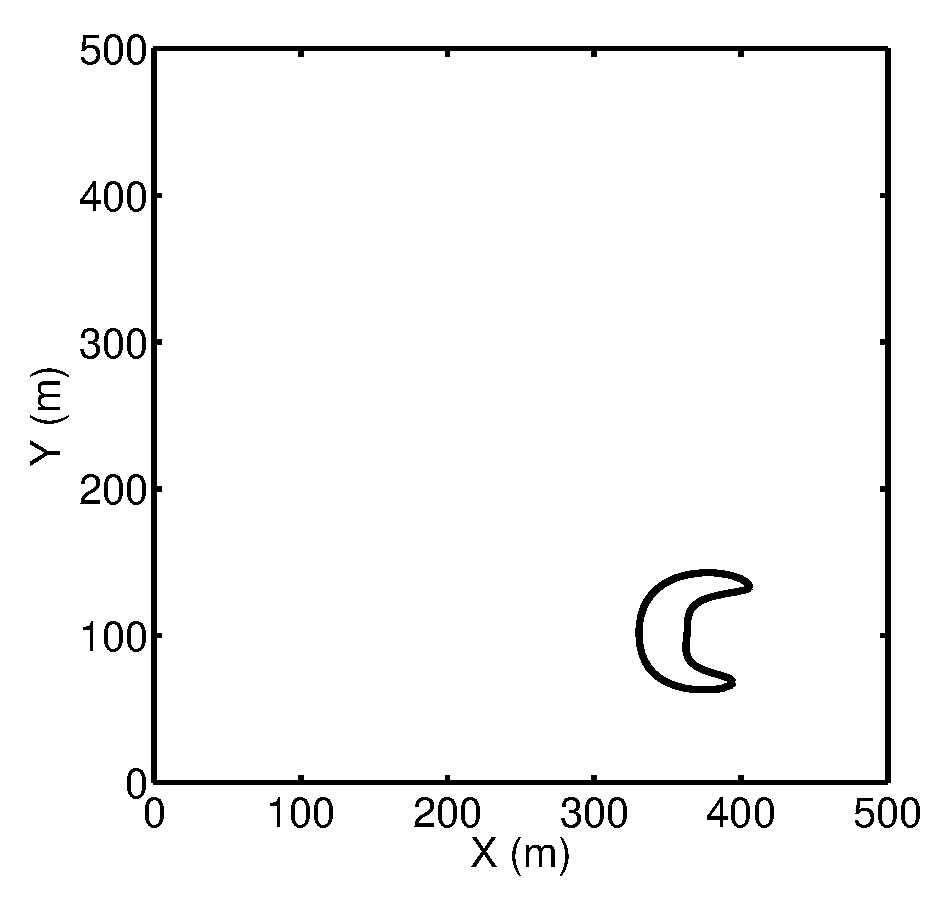
\includegraphics[width=1.3in]{eps/da_data}  &
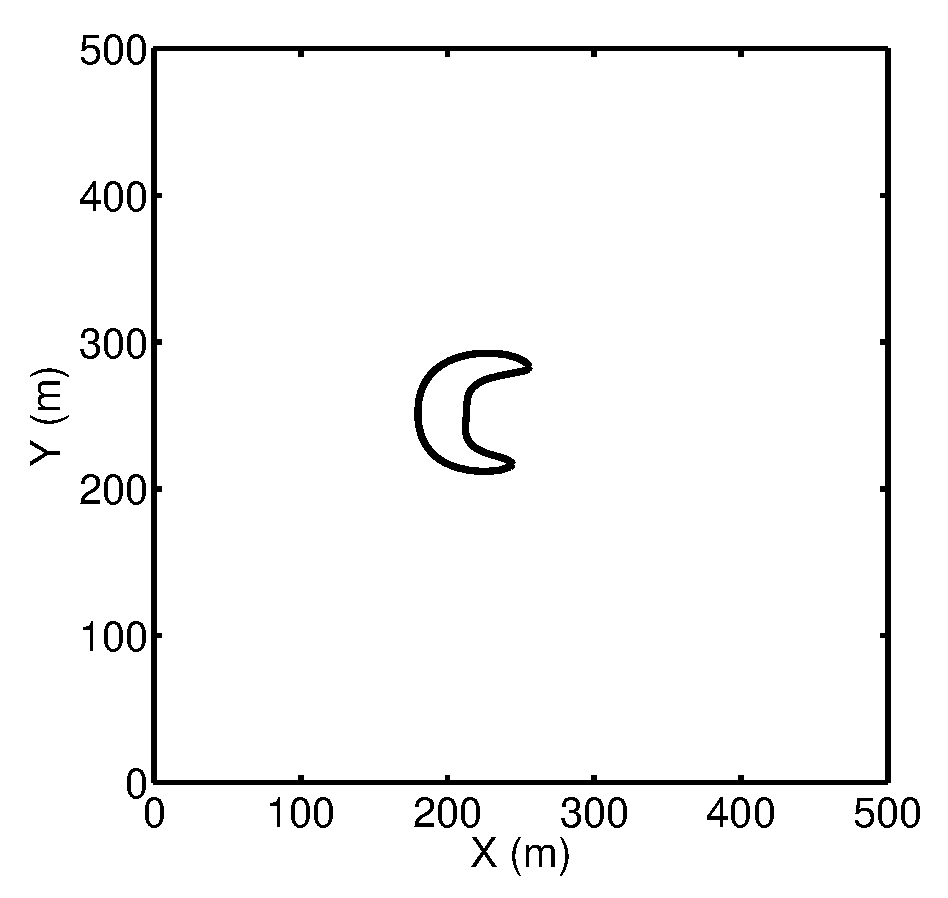
\includegraphics[width=1.3in]{eps/da_fireprofile}\\
Data&Reference\\
%(a) & (b)\\
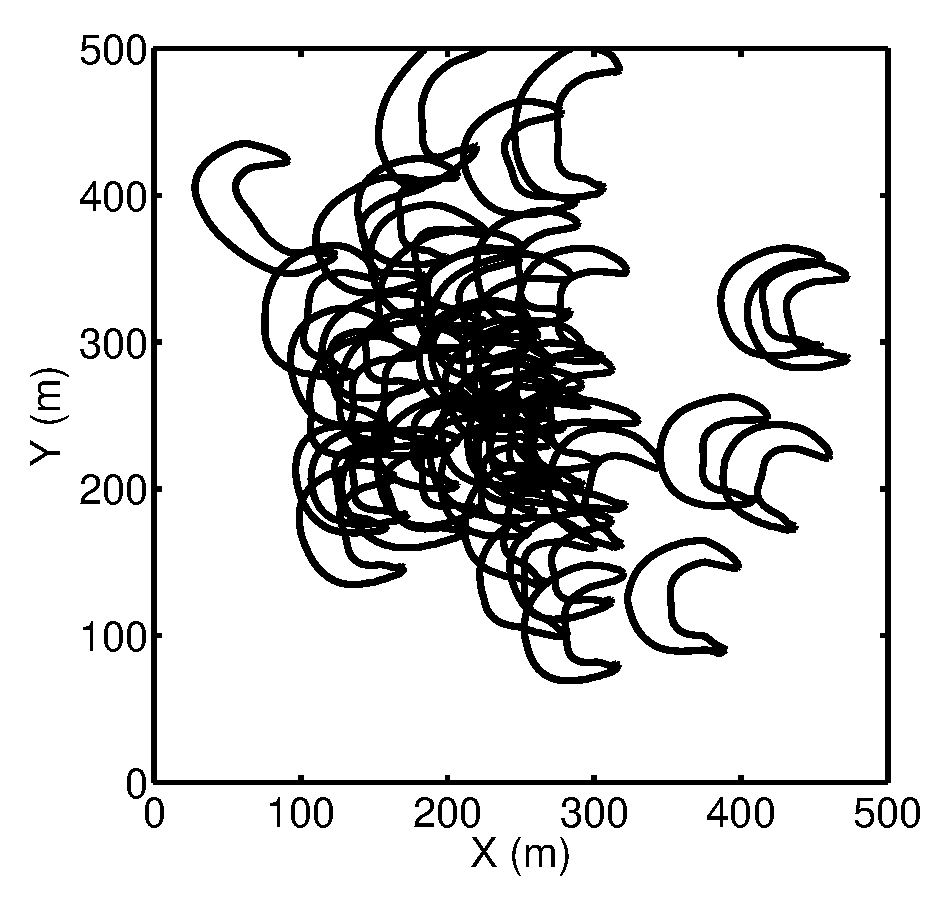
\includegraphics[width=1.3in]{eps/da_prior} &
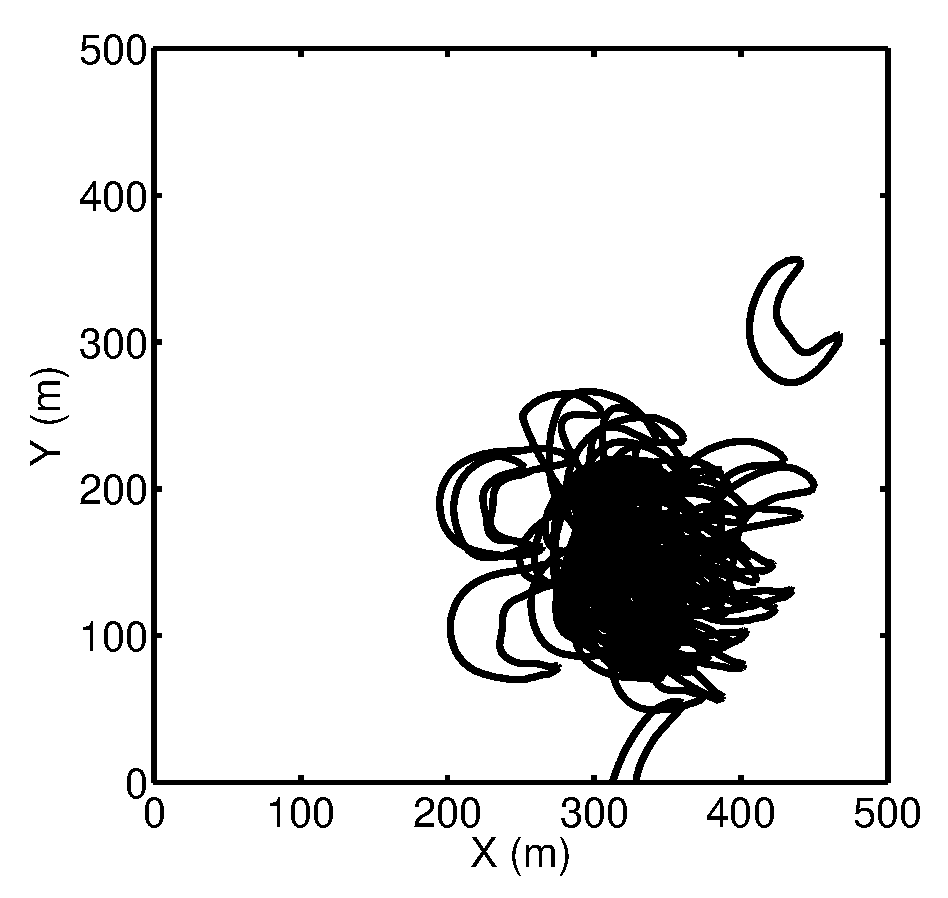
\includegraphics[width=1.3in]{eps/da_posterior}\\
Forecast Ensemble&Analysis Ensemble
%(c) & (d)
\end{tabular}
\newline
\end{center}
\end{figure}

\end{frame}

\begin{frame}
%\frametitle{Computational results}
\vspace{-.1in}
\begin{figure}[t!]
\begin{center}%
\begin{tabular}
[c]{cc}%
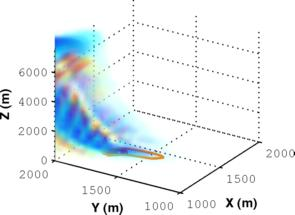
\includegraphics[width=1.8in]{eps/wrf_obs}  &
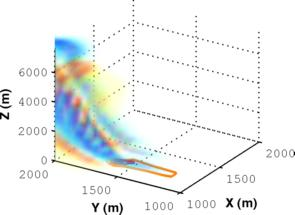
\includegraphics[width=1.8in]{eps/wrf_comp}\\
Data&Reference\\
%(a) & (b)\\
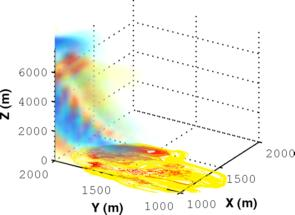
\includegraphics[width=1.8in]{eps/wrf_std} &
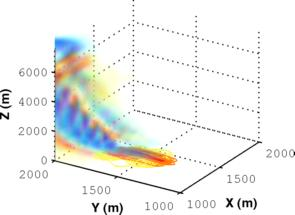
\includegraphics[width=1.8in]{eps/wrf_post}\\
Standard EnKF&Morphing EnKF
%(c) & (d)
\end{tabular}
\newline
\end{center}

\end{figure}

\end{frame}

\end{document}
